\documentclass[a4paper,10pt]{article}


%opening
\title{}
\author{}

\begin{document}

\section{Introduction}

YardSale is an open source Point of Sale system that is being designed by A.S Logic Systems to revolutionize the way Point of Sale systems are implemented in today's market.  Current implementations of Point of Sale systems are fraught with a number of issues; including often being extremely overpriced, difficult to administer, dated in their functionality, and lacking necessary operations.  YardSale was designed to alleviate these problems and allow for extensibility as the market of retail sale expands in the future.

Being that YardSale is an open source project with little funding, the initial niche market will target small, locally owned retail stores.  This type of market will allow for extensive on-site research, as many of these businesses should be willing to work with us to improve on the functionality of their existing POS system.  In addition, because A.S. Logic has decided to take the open source route, the software itself will be freely available to all who wish to use it, the only expense that will come into play is if the company wishes to enlist our services in setup, troubleshooting, support, expansion, or customization.

\section{Functional Requirements}

\subsection{Overview}

This section entails all of the minimal requirements set by the AS Logic Systems development team for the OpenPOS hereafter referred to as YardSale.\\
\\
YardSale at its most minimal functionality level should accomplish the following goals:

\begin{itemize}
	\item {Manage Inventory Data}
	\item {Manage Customer Data}
	\item {Manage Employee Data}
	\item {Perform Transactions}
	\item {Provide Logging Facilities}
	\item {Report on Data}
\end{itemize}

Each of these tasks is described in depth in their corresponding sub sections. There is planned functionality above and beyond this basic featureset, although without these functions other functionality can not be added.

\subsection{Database Management}

The goal of the database management tasks is to add, modify, and delete information in the database. The database backend will run on a MySQL server and all relevant data will be stored in its own table or set of tables. More information on the database design can be found in the database design document.

The inventory management system will have an interface for the stock employees to enter new shipments. It will also have an interface for the management employees to define new items for sale. The most common use of the inventory management system will be integrated into the checkout system. When customers are checking out, inventory will be populated to the checkout screen from the database, and then decremented on purchase from their quantity in the database.

The customer management system will work in a similar fashion to the inventory management system. It will have only one level of functionality though, the ability to define and update new customer data. There will also be a small interface with the database during the checkout of a customer which will allow for the selection of a customer from the customer table.

The employee management system here again will also function similarly to the previous two in that it has hooks into the database for employees. It will allow an authorized user the ability to add and modify employee information as well as disable employee accounts.

Among the more specific functionality of each of these sections would be to allow the user to retrieve any item stored in either inventory, customer, or employee tables given a search criteria. 

\subsection{Transactions}

Transactions in YardSale are basically a 4 step process. The first step in the process is to select a customer to do business with or select a cash "quick" customer. After the customer is selected their basic information will be displayed on the main checkout screen. The user will will then either select items from the inventory from a hierarchy, scan them in with the barcode scanner, or manually type in their information in lookup fields to checkout a customer. A running total will be kept as well as tax calculations for the sale. After all items are accounted for a checkout screen will be called. This will allow the user to select the customer's preferred method of payment and also provide the user with the ability to calculate the correct amount of change.

All transactions will be maintained with a table in the database that will link related elements of the transaction together for later reporting.

\subsection{Logging}

Many program logging features will be provided inherently due to the database backend. Among the logging facilities will be the following items:

\begin{itemize}
\item {Employee Time Tracking}
\item {Transaction Logging}
\item {Shipment Logs}
\item {SQL String Execution Logging}
\end{itemize}

Employee time tracking will be logged based on when the login to their first client and when the logout of their last client. An entry in the Login table will track this for each instance of a session. The transaction logging as was discussed earlier will be maintained in a table of its own tracking related items, customers, and employees with transactions. The shipment logs will be an offshoot of a transaction in that some will be shipped. If so a log of the shipping information will be available as it relates to the customer and the carrier. As a debugging feature a SQL String Execution Log facility will also be included. For every SQL string used on the database, there will be a stored procedure that adds it to the log table for later searching and debug use. This feature will likely be disabled in the final deliverable.

\subsection{Reporting}

There will be a wide variety of reporting features available also as a result of the database backend. The following basic reporting functionality will be available in the first iteration of YardSale.

\begin{itemize}
\item{Payroll for Employees}
\item{Top Sales for Inventory Items}
\item{Top Sales for Employees}
\item{Top Sales for Customer}
\item{Revenue Reporting given any time frame}
\item{Hourly Employee Log Reporting}
\end{itemize}

All of the reports will be outputted to a pdf via \LaTeX type setting. This will provide ease of portability and a wide range of flexibility in reporting.

\section{Design}

This section is still in the works

\section{Implementation}

\subsection{Class Documentation}

Please note the following section was auto-generated. We are working on tweaking this output a little, but currently it is sectioned wrong.

\section{Yard\-Database Class Reference}
\label{classYardDatabase}\index{YardDatabase@{YardDatabase}}
{\tt \#include $<$ys\_\-database.h$>$}

Collaboration diagram for Yard\-Database:\begin{figure}[H]
\begin{center}
\leavevmode
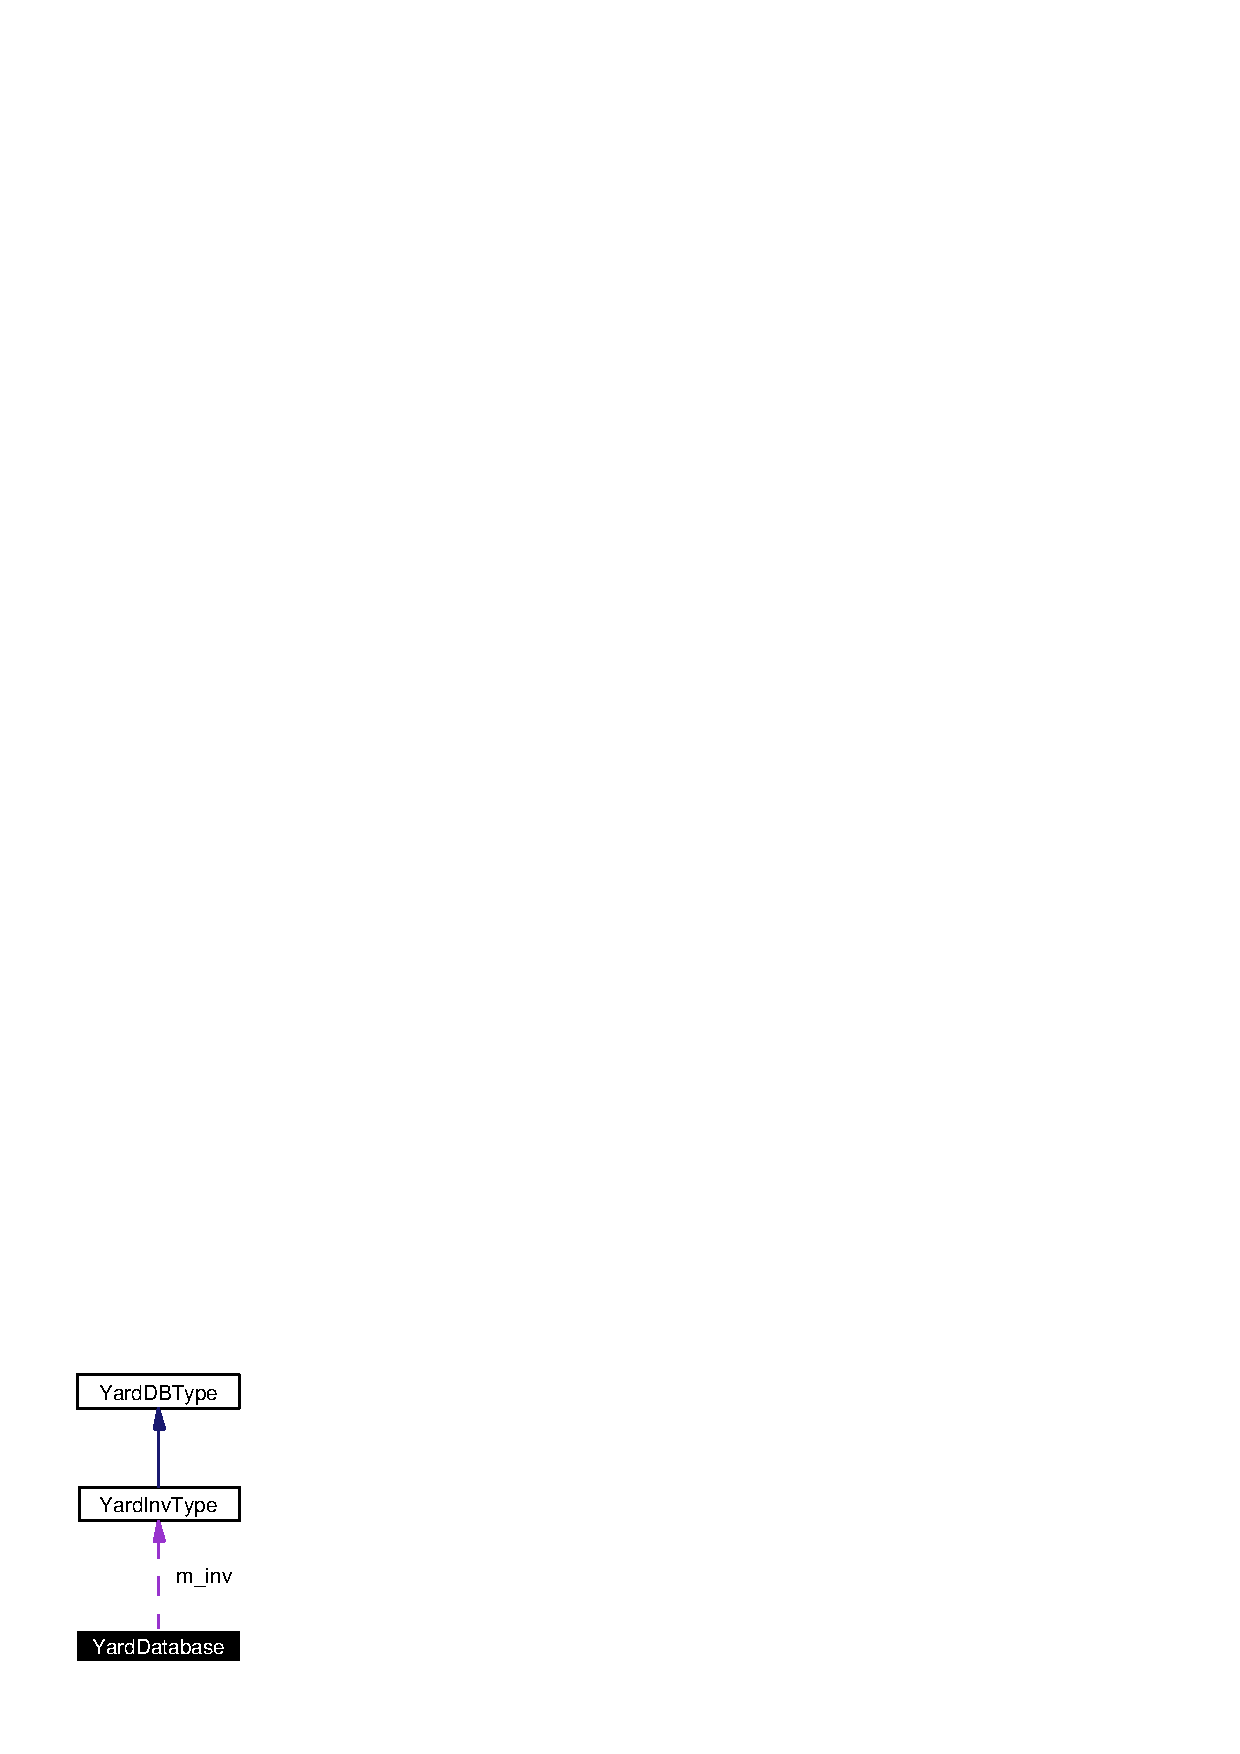
\includegraphics[width=60pt]{classYardDatabase__coll__graph}
\end{center}
\end{figure}


\subsection{Detailed Description}
This is the main database backend which does all translation from OO calls to SQL/ODBC. 

\begin{Desc}
\item[See also:]{\bf Yard\-Inv\-Type}{\rm (p.\,\pageref{classYardInvType})} \end{Desc}


\subsection*{Public Member Functions}
\begin{CompactItemize}
\item 
{\bf Yard\-Database} (const wx\-String \&dsn, const wx\-String \&name, const wx\-String \&pass)\label{classYardDatabase_a0}

\item 
bool {\bf connect} ()\label{classYardDatabase_a2}

\item 
vector$<$ {\bf Yard\-Inv\-Type} $>$ {\bf Inv\-Search\-Keyword} (const unsigned long \&sku)
\begin{CompactList}\small\item\em Find all inventory matches of keyword search. \item\end{CompactList}\item 
vector$<$ {\bf Yard\-Inv\-Type} $>$ {\bf Inv\-Get} (unsigned int num, unsigned int offset)
\begin{CompactList}\small\item\em Get a batch of inventory items. \item\end{CompactList}\end{CompactItemize}


\subsection{Member Function Documentation}
\index{YardDatabase@{Yard\-Database}!InvGet@{InvGet}}
\index{InvGet@{InvGet}!YardDatabase@{Yard\-Database}}
\subsubsection{\setlength{\rightskip}{0pt plus 5cm}vector$<${\bf Yard\-Inv\-Type}$>$ Yard\-Database::Inv\-Get (unsigned int {\em num}, unsigned int {\em offset})}\label{classYardDatabase_a4}


Get a batch of inventory items. 

\begin{Desc}
\item[Parameters:]
\begin{description}
\item[{\em num}]The number of items to get. \item[{\em offset}]The item index to start at. \end{description}
\end{Desc}
\begin{Desc}
\item[Returns:]A std::vector of {\bf Yard\-Inv\-Type}{\rm (p.\,\pageref{classYardInvType})} objects \end{Desc}
\index{YardDatabase@{Yard\-Database}!InvSearchKeyword@{InvSearchKeyword}}
\index{InvSearchKeyword@{InvSearchKeyword}!YardDatabase@{Yard\-Database}}
\subsubsection{\setlength{\rightskip}{0pt plus 5cm}vector$<${\bf Yard\-Inv\-Type}$>$ Yard\-Database::Inv\-Search\-Keyword (const unsigned long \& {\em sku})}\label{classYardDatabase_a3}


Find all inventory matches of keyword search. 

\begin{Desc}
\item[Note:]This could be dangerous, need to limit all returns to some set value (or configured value). \end{Desc}
\begin{Desc}
\item[Parameters:]
\begin{description}
\item[{\em keyword}]A text string to search for. \end{description}
\end{Desc}
\begin{Desc}
\item[Returns:]A std::vector of {\bf Yard\-Inv\-Type}{\rm (p.\,\pageref{classYardInvType})} objects \end{Desc}


The documentation for this class was generated from the following files:\begin{CompactItemize}
\item 
ys\_\-database.h\item 
ys\_\-database.cpp\end{CompactItemize}

\section{Yard\-DBType Class Reference}
\label{classYardDBType}\index{YardDBType@{YardDBType}}
{\tt \#include $<$ys\_\-dbtype.h$>$}

Inheritance diagram for Yard\-DBType:\begin{figure}[H]
\begin{center}
\leavevmode
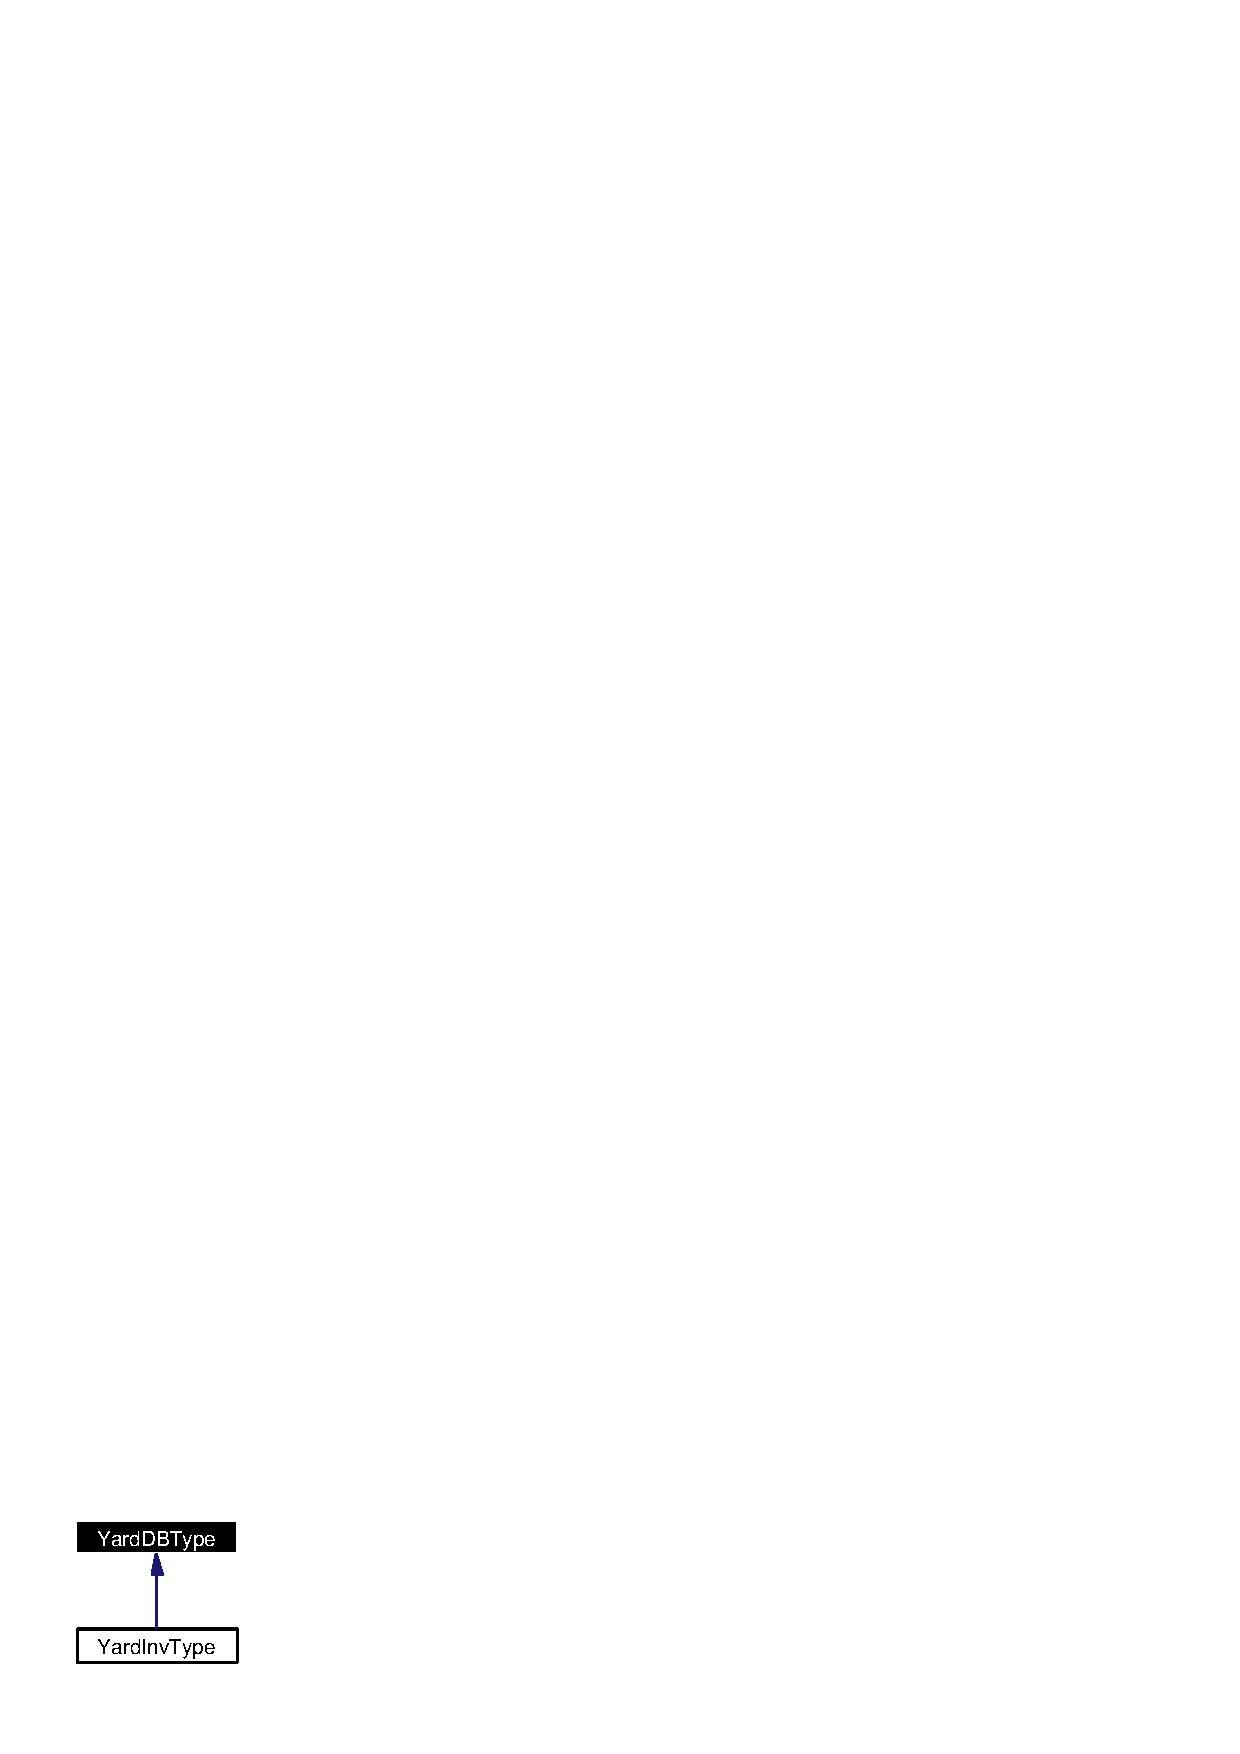
\includegraphics[width=57pt]{classYardDBType__inherit__graph}
\end{center}
\end{figure}


\subsection{Detailed Description}
Abstract base class for datebase objects in {\bf Yard\-Sale}{\rm (p.\,\pageref{classYardSale})}. 

\begin{Desc}
\item[Author:]Jesse Lovelace \end{Desc}


\subsection*{Public Member Functions}
\begin{CompactItemize}
\item 
{\bf Yard\-DBType} (const {\bf Yard\-DBType} \&obj)\label{classYardDBType_a1}

\end{CompactItemize}


The documentation for this class was generated from the following file:\begin{CompactItemize}
\item 
ys\_\-dbtype.h\end{CompactItemize}

\section{Yard\-Employee Class Reference}
\label{classYardEmployee}\index{YardEmployee@{YardEmployee}}
{\tt \#include $<$ys\_\-employee.h$>$}



\subsection{Detailed Description}
Yard\-Employee is the employee managment screen for {\bf Yard\-Sale}{\rm (p.\,\pageref{classYardSale})}. 

Depending on access level, users may insert/modify employee information via this screen. \begin{Desc}
\item[Author:]Jesse Lovelace \end{Desc}


\subsection*{Public Member Functions}
\begin{CompactItemize}
\item 
{\bf Yard\-Employee} (wx\-Window $\ast$parent, wx\-Window\-ID id, const wx\-String \&title, const wx\-Point \&pos=wx\-Default\-Position, const wx\-Size \&size=wx\-Default\-Size, long style=wx\-RESIZE\_\-BORDER)\label{classYardEmployee_a0}

\end{CompactItemize}


The documentation for this class was generated from the following files:\begin{CompactItemize}
\item 
ys\_\-employee.h\item 
ys\_\-employee.cpp\end{CompactItemize}

\section{Yard\-Inventory Class Reference}
\label{classYardInventory}\index{YardInventory@{YardInventory}}
{\tt \#include $<$ys\_\-inventory.h$>$}



\subsection{Detailed Description}
The inventory screen. 

\begin{Desc}
\item[Author:]Jesse Lovelace \end{Desc}
\begin{Desc}
\item[Version:]\begin{Desc}
\item[Revision]1.5 \end{Desc}
\end{Desc}


\subsection*{Public Member Functions}
\begin{CompactItemize}
\item 
{\bf Yard\-Inventory} (wx\-Window $\ast$parent, wx\-Window\-ID id, const wx\-String \&title, const wx\-Point \&pos=wx\-Default\-Position, const wx\-Size \&size=wx\-Default\-Size, long style=wx\-RESIZE\_\-BORDER)\label{classYardInventory_a0}

\item 
void {\bf On\-Exit\-Button} (wx\-Command\-Event \&event)
\begin{CompactList}\small\item\em Exit button handler. \item\end{CompactList}\end{CompactItemize}


\subsection{Member Function Documentation}
\index{YardInventory@{Yard\-Inventory}!OnExitButton@{OnExitButton}}
\index{OnExitButton@{OnExitButton}!YardInventory@{Yard\-Inventory}}
\subsubsection{\setlength{\rightskip}{0pt plus 5cm}void Yard\-Inventory::On\-Exit\-Button (wx\-Command\-Event \& {\em event})}\label{classYardInventory_a2}


Exit button handler. 

\begin{Desc}
\item[Parameters:]
\begin{description}
\item[{\em event}]The event being passed in. \end{description}
\end{Desc}


The documentation for this class was generated from the following files:\begin{CompactItemize}
\item 
ys\_\-inventory.h\item 
ys\_\-inventory.cpp\end{CompactItemize}

\section{Yard\-Inv\-Type Class Reference}
\label{classYardInvType}\index{YardInvType@{YardInvType}}
{\tt \#include $<$ys\_\-inv\_\-type.h$>$}

Inheritance diagram for Yard\-Inv\-Type:\begin{figure}[H]
\begin{center}
\leavevmode
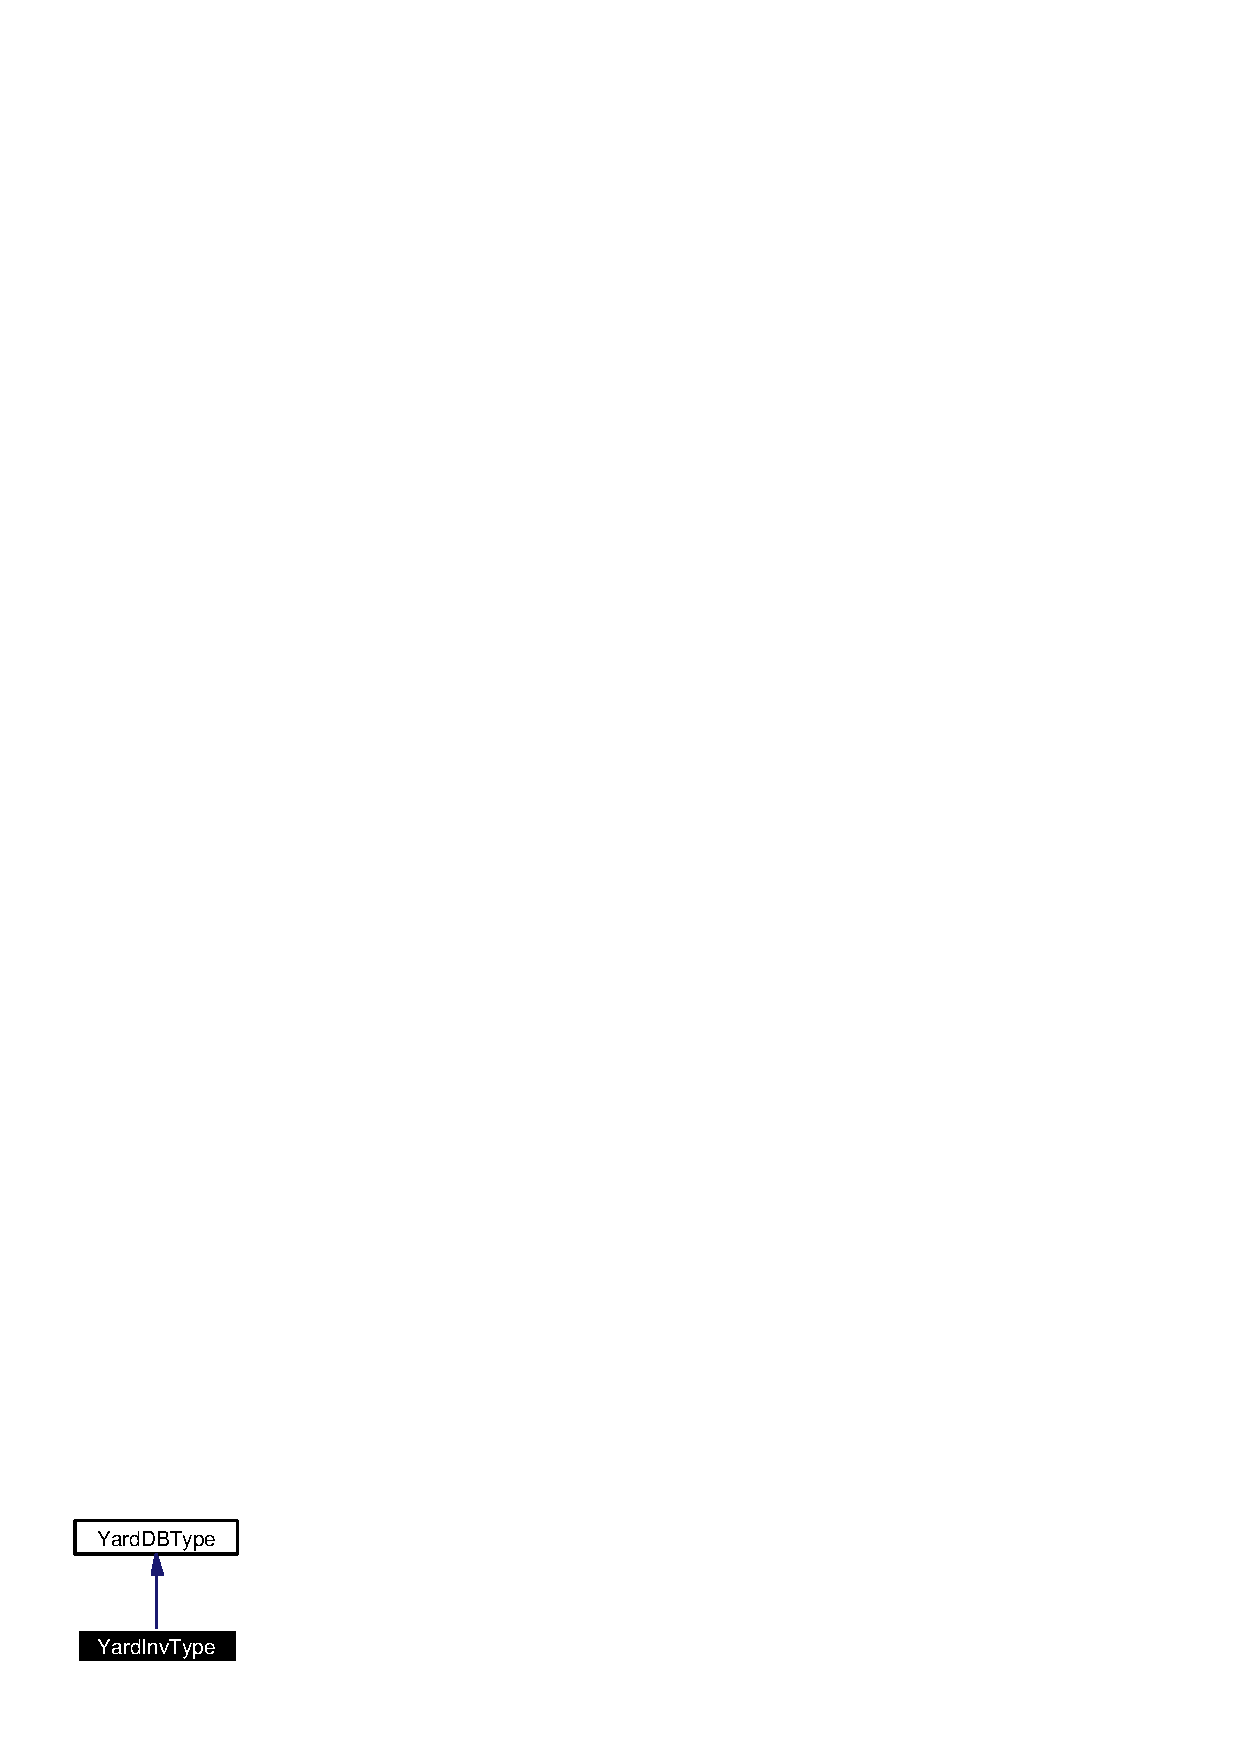
\includegraphics[width=57pt]{classYardInvType__inherit__graph}
\end{center}
\end{figure}
Collaboration diagram for Yard\-Inv\-Type:\begin{figure}[H]
\begin{center}
\leavevmode
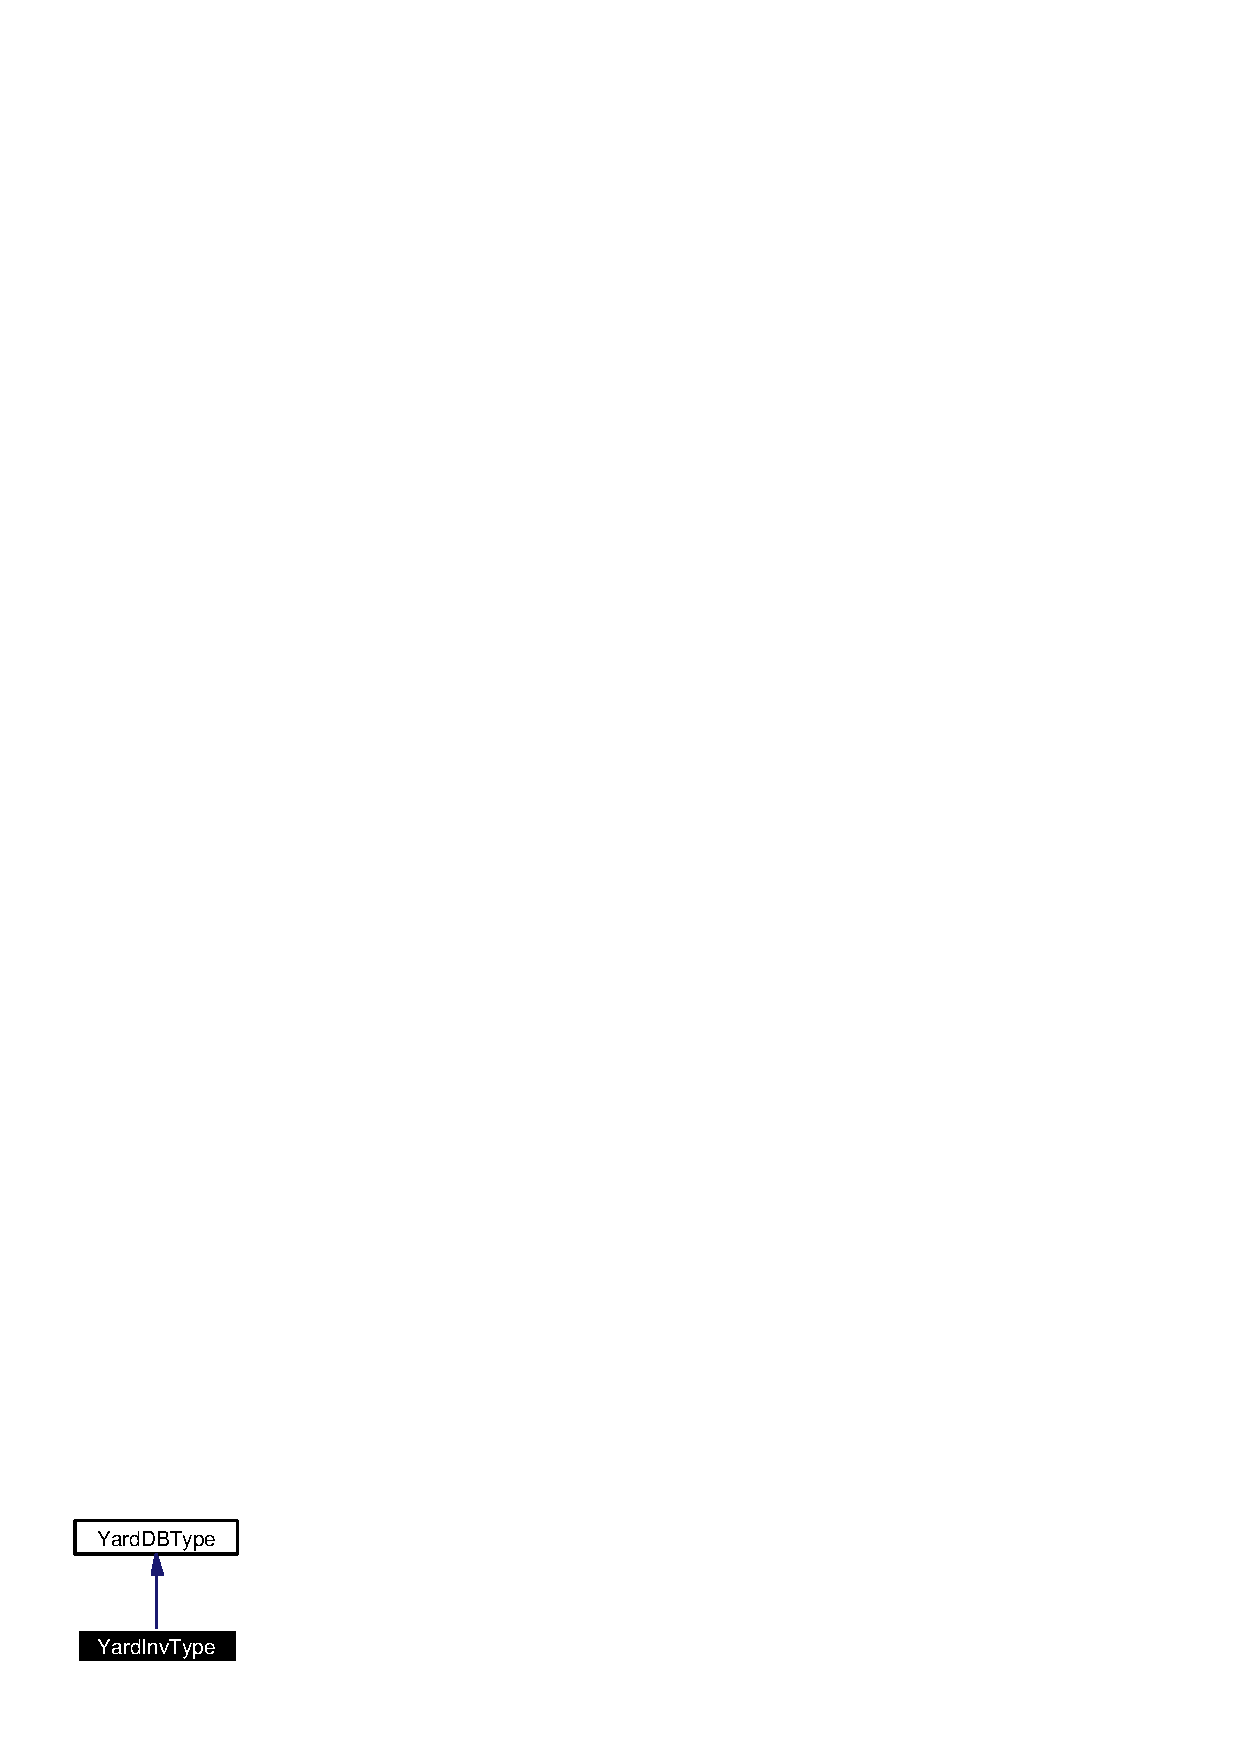
\includegraphics[width=57pt]{classYardInvType__coll__graph}
\end{center}
\end{figure}


\subsection{Detailed Description}
The {\bf Yard\-Sale}{\rm (p.\,\pageref{classYardSale})} Inventory Type is a OO representation of the datebase inventory table. 

\begin{Desc}
\item[Author:]Jesse Lovelace \end{Desc}
\begin{Desc}
\item[Version:]\begin{Desc}
\item[Revision]1.3 \end{Desc}
\end{Desc}
\begin{Desc}
\item[See also:]{\bf Yard\-DBType}{\rm (p.\,\pageref{classYardDBType})} \end{Desc}


\subsection*{Public Member Functions}
\begin{CompactItemize}
\item 
{\bf Yard\-Inv\-Type} (const {\bf Yard\-Inv\-Type} \&obj)\label{classYardInvType_a1}

\begin{CompactList}\small\item\em Copy constructor. \item\end{CompactList}\item 
{\bf Yard\-Inv\-Type} \& {\bf operator=} (const {\bf Yard\-Inv\-Type} \&obj)\label{classYardInvType_a2}

\item 
wx\-String {\bf Get\-Bar\-Code} () const \label{classYardInvType_a3}

\item 
wx\-String {\bf Get\-Description} () const \label{classYardInvType_a4}

\item 
wx\-String {\bf Get\-Department} () const \label{classYardInvType_a5}

\item 
unsigned long {\bf Get\-Quant\-On\-Hand} () const \label{classYardInvType_a6}

\item 
unsigned long {\bf Get\-Quant\-On\-Order} () const \label{classYardInvType_a7}

\item 
unsigned long {\bf Get\-Reorder\-Level} () const \label{classYardInvType_a8}

\item 
wx\-String {\bf Get\-Item\-Type} () const \label{classYardInvType_a9}

\item 
float {\bf Get\-Item\-Weight\-Lbs} () const \label{classYardInvType_a10}

\item 
float {\bf Get\-Tax\-Type} () const \label{classYardInvType_a11}

\item 
long int {\bf Get\-Vendor\-Id} () const \label{classYardInvType_a12}

\item 
float {\bf Get\-Retail\-Price} () const \label{classYardInvType_a13}

\item 
float {\bf Get\-Wholesale\-Price} () const \label{classYardInvType_a14}

\item 
vector$<$ Bulk\-Pricing $>$ {\bf Get\-Bulk\-Pricing} () const \label{classYardInvType_a15}

\item 
bool {\bf Is\-Over\-Sized} () const \label{classYardInvType_a16}

\item 
bool {\bf Must\-Ship\-Freight} () const \label{classYardInvType_a17}

\item 
void {\bf Set\-Bar\-Code} (const wx\-String \&str)\label{classYardInvType_a18}

\item 
void {\bf Set\-Description} (const wx\-String \&str)\label{classYardInvType_a19}

\item 
void {\bf Set\-Department} (const wx\-String \&str)\label{classYardInvType_a20}

\item 
void {\bf Set\-Quant\-On\-Hand} (unsigned long num)\label{classYardInvType_a21}

\item 
void {\bf Set\-Quant\-On\-Order} (unsigned long num)\label{classYardInvType_a22}

\item 
void {\bf Set\-Reorder\-Level} (unsigned long num)\label{classYardInvType_a23}

\item 
void {\bf Set\-Item\-Type} (const wx\-String \&str)\label{classYardInvType_a24}

\item 
void {\bf Set\-Item\-Weight\-Lbs} (float num)\label{classYardInvType_a25}

\item 
void {\bf Set\-Tax\-Type} (float num)\label{classYardInvType_a26}

\item 
void {\bf Set\-Ventor\-Id} (long int num)\label{classYardInvType_a27}

\item 
void {\bf Set\-Retail\-Price} (float num)\label{classYardInvType_a28}

\item 
void {\bf Set\-Wholesale\-Price} (float num)\label{classYardInvType_a29}

\item 
bool {\bf Add\-Bulk\-Price} (const Bulk\-Pricing \&price)\label{classYardInvType_a30}

\item 
bool {\bf Remove\-Bulk\-Price} (unsigned int level)\label{classYardInvType_a31}

\item 
void {\bf Set\-Over\-Sized} (bool cond)\label{classYardInvType_a32}

\item 
void {\bf Set\-Ship\-Freight} (bool cond)\label{classYardInvType_a33}

\end{CompactItemize}
\subsection*{Friends}
\begin{CompactItemize}
\item 
class {\bf Yard\-Database}\label{classYardInvType_n0}

\end{CompactItemize}


The documentation for this class was generated from the following files:\begin{CompactItemize}
\item 
ys\_\-inv\_\-type.h\item 
ys\_\-inv\_\-type.cpp\end{CompactItemize}

\section{Yard\-Login Class Reference}
\label{classYardLogin}\index{YardLogin@{YardLogin}}
{\tt \#include $<$ys\_\-login.h$>$}



\subsection{Detailed Description}
This is the customized login screen for {\bf Yard\-Sale}{\rm (p.\,\pageref{classYardSale})}. 

\begin{Desc}
\item[Author:]Jesse Lovelace \end{Desc}
\begin{Desc}
\item[Version:]\begin{Desc}
\item[Revision]1.3 \end{Desc}
\end{Desc}


\subsection*{Public Member Functions}
\begin{CompactItemize}
\item 
{\bf Yard\-Login} (wx\-Window $\ast$parent, wx\-Window\-ID id, const wx\-String \&title, const wx\-Point \&pos=wx\-Default\-Position, const wx\-Size \&size=wx\-Default\-Size, long style=wx\-STAY\_\-ON\_\-TOP$|$wx\-RESIZE\_\-BORDER)\label{classYardLogin_a0}

\item 
void {\bf On\-Exit\-Button} (wx\-Command\-Event \&event)
\begin{CompactList}\small\item\em Exit button handler. \item\end{CompactList}\item 
void {\bf On\-Login} (wx\-Command\-Event \&event)\label{classYardLogin_a3}

\end{CompactItemize}


\subsection{Member Function Documentation}
\index{YardLogin@{Yard\-Login}!OnExitButton@{OnExitButton}}
\index{OnExitButton@{OnExitButton}!YardLogin@{Yard\-Login}}
\subsubsection{\setlength{\rightskip}{0pt plus 5cm}void Yard\-Login::On\-Exit\-Button (wx\-Command\-Event \& {\em event})}\label{classYardLogin_a2}


Exit button handler. 

\begin{Desc}
\item[Parameters:]
\begin{description}
\item[{\em event}]The event being passed in. \end{description}
\end{Desc}


The documentation for this class was generated from the following files:\begin{CompactItemize}
\item 
ys\_\-login.h\item 
ys\_\-login.cpp\end{CompactItemize}

\section{Yard\-Main Class Reference}
\label{classYardMain}\index{YardMain@{YardMain}}
{\tt \#include $<$ys\_\-main.h$>$}



\subsection{Detailed Description}
Yard\-Main is the main menu screen for {\bf Yard\-Sale}{\rm (p.\,\pageref{classYardSale})}, it displays graphical buttons for accessing the inventory, employees, sales, etc. 

\begin{Desc}
\item[Author:]Jesse Lovelace \end{Desc}
\begin{Desc}
\item[Version:]\begin{Desc}
\item[Revision]1.6 \end{Desc}
\end{Desc}


\subsection*{Public Member Functions}
\begin{CompactItemize}
\item 
{\bf Yard\-Main} (wx\-Window $\ast$parent, wx\-Window\-ID id, const wx\-String \&title, const wx\-Point \&pos=wx\-Default\-Position, const wx\-Size \&size=wx\-Default\-Size, long style=wx\-RESIZE\_\-BORDER$|$wx\-FRAME\_\-NO\_\-TASKBAR)
\begin{CompactList}\small\item\em Constructor. \item\end{CompactList}\item 
void {\bf On\-Logout} (wx\-Command\-Event \&event)\label{classYardMain_a2}

\begin{CompactList}\small\item\em Logout button event handler. \item\end{CompactList}\item 
void {\bf On\-Max} (wx\-Command\-Event \&event)\label{classYardMain_a3}

\begin{CompactList}\small\item\em Maximize handler. \item\end{CompactList}\item 
void {\bf On\-Inventory} (wx\-Command\-Event \&event)\label{classYardMain_a4}

\begin{CompactList}\small\item\em Inventory button handler. \item\end{CompactList}\item 
void {\bf On\-Sale} (wx\-Command\-Event \&event)\label{classYardMain_a5}

\begin{CompactList}\small\item\em Sales buttons. \item\end{CompactList}\item 
void {\bf On\-Employee} (wx\-Command\-Event \&event)\label{classYardMain_a6}

\begin{CompactList}\small\item\em Employee button handler. \item\end{CompactList}\end{CompactItemize}


\subsection{Constructor \& Destructor Documentation}
\index{YardMain@{Yard\-Main}!YardMain@{YardMain}}
\index{YardMain@{YardMain}!YardMain@{Yard\-Main}}
\subsubsection{\setlength{\rightskip}{0pt plus 5cm}Yard\-Main::Yard\-Main (wx\-Window $\ast$ {\em parent}, wx\-Window\-ID {\em id}, const wx\-String \& {\em title}, const wx\-Point \& {\em pos} = wx\-Default\-Position, const wx\-Size \& {\em size} = wx\-Default\-Size, long {\em style} = wx\-RESIZE\_\-BORDER$|$wx\-FRAME\_\-NO\_\-TASKBAR)}\label{classYardMain_a0}


Constructor. 



\begin{Desc}
\item[{\bf Todo}]Make these compiled into the binary.\end{Desc}


The documentation for this class was generated from the following files:\begin{CompactItemize}
\item 
ys\_\-main.h\item 
ys\_\-main.cpp\end{CompactItemize}

\section{Yard\-Sale Class Reference}
\label{classYardSale}\index{YardSale@{YardSale}}
{\tt \#include $<$yardsale.h$>$}



\subsection{Detailed Description}
This is the main application object. 

\begin{Desc}
\item[Author:]Jesse Lovelace \end{Desc}
\begin{Desc}
\item[Version:]\begin{Desc}
\item[Revision]1.8 \end{Desc}
\end{Desc}


\subsection*{Public Member Functions}
\begin{CompactItemize}
\item 
virtual bool {\bf On\-Init} ()
\begin{CompactList}\small\item\em This is the function were top level windows are created. \item\end{CompactList}\end{CompactItemize}


\subsection{Member Function Documentation}
\index{YardSale@{Yard\-Sale}!OnInit@{OnInit}}
\index{OnInit@{OnInit}!YardSale@{Yard\-Sale}}
\subsubsection{\setlength{\rightskip}{0pt plus 5cm}bool Yard\-Sale::On\-Init ()\hspace{0.3cm}{\tt  [virtual]}}\label{classYardSale_a0}


This is the function were top level windows are created. 

\begin{Desc}
\item[Returns:]True if application initialized ok \end{Desc}


The documentation for this class was generated from the following files:\begin{CompactItemize}
\item 
yardsale.h\item 
yardsale.cpp\end{CompactItemize}

\section{Yard\-Sale\-Screen Class Reference}
\label{classYardSaleScreen}\index{YardSaleScreen@{YardSaleScreen}}
{\tt \#include $<$ys\_\-sale.h$>$}



\subsection{Detailed Description}
This is the main sale screen. 

It contains the current transaction information. \begin{Desc}
\item[Author:]Jesse Lovelace \end{Desc}
\begin{Desc}
\item[Version:]\begin{Desc}
\item[Revision]1.3 \end{Desc}
\end{Desc}


\subsection*{Public Member Functions}
\begin{CompactItemize}
\item 
{\bf Yard\-Sale\-Screen} (wx\-Window $\ast$parent, wx\-Window\-ID id, const wx\-String \&title, const wx\-Point \&pos=wx\-Default\-Position, const wx\-Size \&size=wx\-Default\-Size, long style=wx\-RESIZE\_\-BORDER)\label{classYardSaleScreen_a0}

\item 
void {\bf On\-Exit\-Button} (wx\-Command\-Event \&event)\label{classYardSaleScreen_a2}

\begin{CompactList}\small\item\em Exit button event handler. \item\end{CompactList}\end{CompactItemize}


The documentation for this class was generated from the following files:\begin{CompactItemize}
\item 
ys\_\-sale.h\item 
ys\_\-sale.cpp\end{CompactItemize}

\section{Yard\-Splash Class Reference}
\label{classYardSplash}\index{YardSplash@{YardSplash}}
{\tt \#include $<$ys\_\-splash.h$>$}



\subsection{Detailed Description}
Eye-candy splash screen. 

\begin{Desc}
\item[Author:]Jesse Lovelace \end{Desc}
\begin{Desc}
\item[Version:]\begin{Desc}
\item[Revision]1.6 \end{Desc}
\end{Desc}


\subsection*{Public Member Functions}
\begin{CompactItemize}
\item 
{\bf Yard\-Splash} (wx\-Window $\ast$parent, wx\-Window\-ID id, const wx\-String \&title, const wx\-Point \&pos=wx\-Default\-Position, const wx\-Size \&size=wx\-Default\-Size, long style=wx\-STAY\_\-ON\_\-TOP)\label{classYardSplash_a0}

\item 
void {\bf On\-Click} (wx\-Mouse\-Event \&event)
\begin{CompactList}\small\item\em Mouse click event handler. \item\end{CompactList}\item 
void {\bf On\-Timer} (wx\-Timer\-Event \&event)\label{classYardSplash_a3}

\begin{CompactList}\small\item\em Timer event handler. \item\end{CompactList}\item 
void {\bf Bump} (unsigned int amount=10)
\begin{CompactList}\small\item\em Called to nudge progress bar over. \item\end{CompactList}\end{CompactItemize}


\subsection{Member Function Documentation}
\index{YardSplash@{Yard\-Splash}!Bump@{Bump}}
\index{Bump@{Bump}!YardSplash@{Yard\-Splash}}
\subsubsection{\setlength{\rightskip}{0pt plus 5cm}void Yard\-Splash::Bump (unsigned int {\em amount} = 10)}\label{classYardSplash_a4}


Called to nudge progress bar over. 

\begin{Desc}
\item[Parameters:]
\begin{description}
\item[{\em amount}]Number of pixels to nudge \end{description}
\end{Desc}
\index{YardSplash@{Yard\-Splash}!OnClick@{OnClick}}
\index{OnClick@{OnClick}!YardSplash@{Yard\-Splash}}
\subsubsection{\setlength{\rightskip}{0pt plus 5cm}void Yard\-Splash::On\-Click (wx\-Mouse\-Event \& {\em event})}\label{classYardSplash_a2}


Mouse click event handler. 

\begin{Desc}
\item[{\bf Deprecated}]This handler is for testing only and will be removed \end{Desc}


The documentation for this class was generated from the following files:\begin{CompactItemize}
\item 
ys\_\-splash.h\item 
ys\_\-splash.cpp\end{CompactItemize}


\section{Test Plan}

\end{document}
